\section{Methodology} 
The methodology section describes the key components of the Transformer-based translation model, including data and model architecture (see \cref{fig:transformer}).

\subsection{Data Preprocessing}
Before the model can process the input data, the data has to be encoded in a numerical representation that the model can interpret.
For this, a shared tokenizer is trained over the source and target sequences, which maps a token (a word or subword) of a sequence to a number and vice versa. 
Correctly aligning the sequences was particularly challenging and required multiple iterations to get right.
A key indicator of misalignment was that the training loss converged to zero, while the validation loss remained high, suggesting poor generalization to unseen data.
This led me to realize that the model was learning to always predict the token it was erroneously able to look at.

\begin{figure}[h]
    \begin{center}
        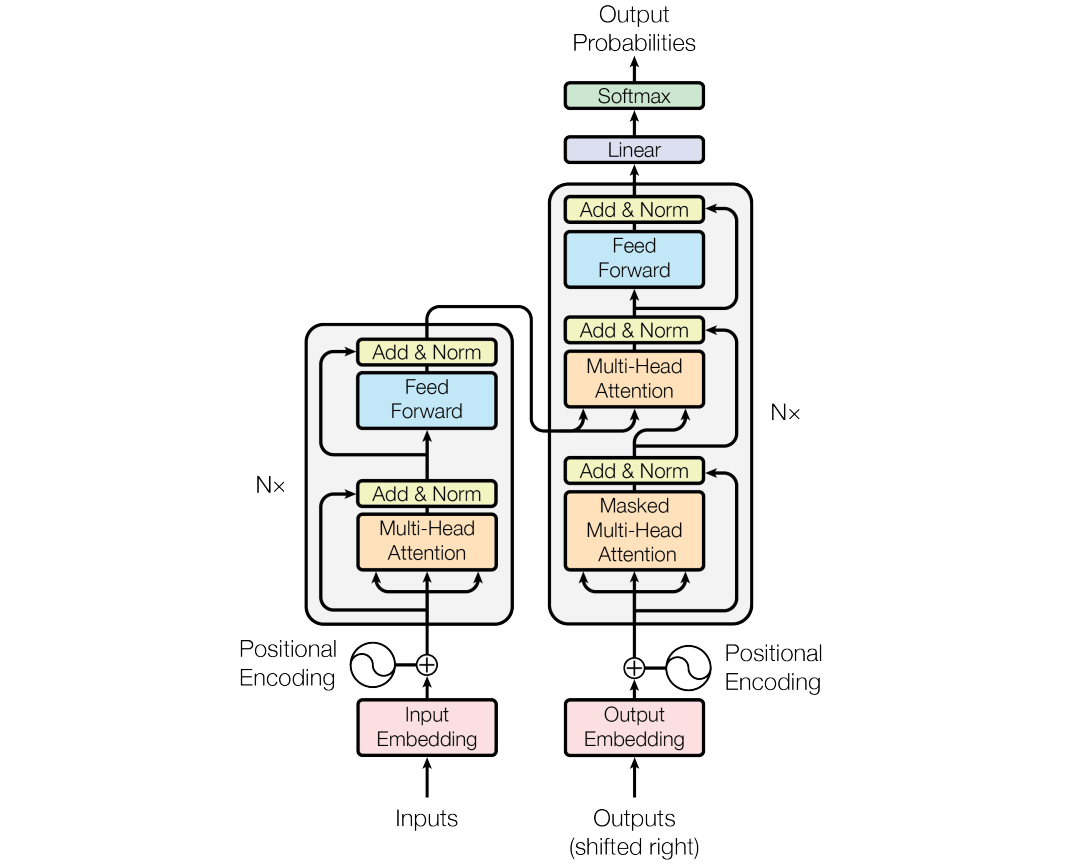
\includegraphics[width=\textwidth]{figures/transformer.png}
    \end{center}
    \caption{The original transformer architecture, adapted from Vaswani et al.~\cite{vaswani2017attention}}\label{fig:transformer}
\end{figure}

\subsection{Embedding Layers} 
After the data is correctly preprocessed, the embedding layer creates a \texttt{$d_{model}$}-dimensional vector representation for each encoded token of the input and target sequence. 
Consistent with the original Transformer architecture, we apply parameter sharing by using the same set of weights for both embedding layers and the pre-softmax linear transformation, which maps the embeddings back to their respective token index.
Sharing parameters between the encoder and decoder embedding layers offers several advantages.
First, it can significantly reduce the model size while maintaining model performance~\cite{press2017usingoutputembeddingimprove}.
Second, parameter sharing reduces the degrees of freedom of the model, thus implicitly applying regularization by forcing different parts of the model to use the same parameters, preventing the model from overfitting.
Additionally, the efficiency of the model improves because shared parameters allow for faster updates and fewer memory operations.
Unlike recurrent architectures, which process sequences step by step, the Transformer processes entire sequences in parallel. 
To compensate for the lack of sequence order awareness, the positional encoding layer enriches the representations with fixed positional information.

\subsection{Encoder Stack} 
The encoder consists of six identical layers, each designed to transform the input sequence into a context-rich representation.
Each layer comprises two sub-layers: a multi-head self-attention mechanism (\cref{sec:attention}) and a position-wise feed-forward network (\cref{sec:ffn}), each followed by a residual connection~\cite{he2015deepresiduallearningimage} and layer normalization~\cite{ba2016layernormalization} (\cref{sec:normalization}) to stabilize training and improve gradient flow.\\
Residual connections, defined as  \(y = \mathbf{x} + f(\mathbf{x})\), preserve the original signal while adding important features from multi-head attention or feed-forward layers, alleviating the problem of vanishing gradients during backpropagation.
If the transformation \(f(\mathbf{x})\) collapses to zero (e.g. due to all weights and biases being pushed to zero), the output reduces to \(y = \mathbf{x}\), ensuring that the original signal is preserved when the layer does not learn anything.
Residual connections can also be described by the residual mapping \(g(\mathbf{x}) = f(\mathbf{x}) - \mathbf{x}\), emphasizing that the network only needs to learn a small transformation when \(f(\mathbf{x})\) is close to the identity function.
Learning a function close to the identity function, residual blocks slightly refine existing features instead of learning full (high variance) functions from scratch. \\

\subsection{Decoder Stack} 
The decoder also consists of six identical layers.
In addition to the two sub-layers of the encoder, it has a second multi-head attention mechanism over the outputs of the encoder.
Consistent with the encoder, residual connections and layer normalization are employed after each sub-layer.
In contrast to the multi-head self-attention layer in the encoder, the inputs to the attention mechanism in the decoder are masked such that the decoder cannot attend to future tokens.
This prevents the decoder from cheating by attending to tokens it has not yet seen.
Finally, the output of the decoder undergoes a linear transformation. After that, softmax is applied to convert the output into probabilities to predict the next token.

% Add how the heads are concatenated in attention
\subsection{Attention}\label{sec:attention}
The attention function injects contextual information about related tokens into each token's representation.
This process enables the model to capture dependencies between words, regardless of their position in the sequence. \\
The first step is to create the query(\(Q)\), key(\(K)\), and value(\(V)\) vectors from the encoder or decoder input vectors by multiplying them with three matrices that are learned during training.
These matrices must be learned in a way that they reflect meaningful similarity relationships in terms of attention.
To ensure that attention is applied correctly, two types of masks are used: a padding mask, which prevents attention from being applied to padding tokens, and a causal mask, which ensures that in the decoder, attention cannot be applied to future tokens.\\
According to \cref{eq:attention}, the attention function then first computes a score for each token in the sequence relative to every other token by taking the dot product of the query vector with the transposed key vector:
\begin{equation}
    \text{Attention}(Q,K,V) = \text{softmax}\left(\frac{QK^T}{\sqrt{d_k}}\right)V
    \label{eq:attention}
\end{equation}
This computation, along with all other operations of the attention mechanism, is performed in parallel for all tokens in each sequence across the entire batch.
Next, the result is scaled by \(\sqrt{d_k}\) to avoid exploding gradients and improve stability.
Then a softmax function is applied to maintain relevant words, subside words we can mostly ignore, and prepare the output to be summed up.
Finally, by multiplying the softmax scores by \(V\) produces a new representation for each token.
While it retains most of its original structure, it is enriched with contextual information form the most relevant tokens for our translation task. \\

\subsection{Position-Wise Feed-Forward Networks} \label{sec:ffn}
According to \cref{eq:ffn}, the FFN introduces a higher-dimensional space to explore non-linear combinations of features present in the token embeddings that it could not explore in the original embedding space:
\begin{equation}\label{eq:ffn}
	\text{FFN}(x) = \max(0, xW_1 + b_1)W_2 + b_2
\end{equation}
That happens by the first linear transformation \(xW_1 + b_1\).
Next, \(\max(0, xW_1 + b_1)\) (ReLU) introduces non-linearity.
The FFN has two linear layers of size \(\left(d_{\text{model}}, d_{\text{ffn}}\right)\) and \(\left(d_{\text{ffn}}, d_{\text{model}}\right)\), respectively.
Finally, the non-linearly transformed representation is projected back into the original space, \(d_{\text{model}}\), such that the model is forced to focus on the most significant feature combinations.

\subsection{Normalization Layer} \label{sec:normalization}
Layer normalization is applied after each self-attention and feed-forward sublayer according to \cref{eq:normalization}:
\begin{equation}\label{eq:normalization}
    \text{LayerNorm}(x) = \frac{x - \mu}{\sigma} \cdot \gamma + \beta \text{,}
\end{equation}
where \(x\) is the input vector, in our case the token embedding, \(\mu\) the mean of \(x\), calculated across the features, \(\sigma\) is the standard deviation, also calculated across the features:
\begin{align}
	\mu^l = \frac{1}{H} \sum_{i=1}^H a_i^l &   & \sigma^l = \sqrt{\frac{1}{H}\sum_{i=1}^H (a_i^l - \mu^l)^2} 
\end{align}
\(H\) is the number of features for each token representation, \(\gamma\) and \(\beta\) are optional, learnable parameters to scale and shift the normalized values. \\
In a transformer architecture, the layer normalization layer serves different purposes: it stabilizes training by normalizing the distributions of the layer inputs, thus preventing exploding or vanishing gradients, which would also have adverse, covariate effects on the surrounding layers in the forward and backward passes.
Additionally, contrary to batch normalization, layer normalization handles variations in sequence length better, since it computes the mean and variance along the features of the token and not across the individual features across the batch.

